%Introduction
\chapter{Introduction}
TODO CHANGE these paragraphs to argue more for the limitations of control systems relying on fixed data - instead discuss how they NEED accurate forecasts.  Perhaps discuss freeway traffic control lights and filling up the freeways if miss timed.


According to the U.S. Department of Energy \cite{DOE2010} energy for heating and cooling accounts for approximately 35 - 45\% of the total expenditure within a building.  With such a large investment of energy being used to regulate the temperature of a building, possible areas of improvement are heavily sought after.  Fully automated buildings with control systems to automatically heat and cool individual rooms or spaces have been designed \cite{Controls2013, Controls2013a} to reduce building energy usage while maintaining proper temperatures throughout the building.  These systems are complex and require knowledge of room usage, and in more complex systems room occupancy, as inputs into system control models.
	
While many factors such as ambient temperature, ventilation air flow, room volume, etc. affect the time it takes to heat or air condition a room, it still takes on the order of many minutes to bring a room to a stable desired temperature \cite{yang2004}.  Due to this lag in changing the temperature of a room, it is not sufficient for control systems to begin air conditioning a room upon initial occupancy.   Thus, to ensure that room temperatures are appropriate, smart building control systems typically rely on set schedules of occupancy.  These systems may use scheduled occupancy unto 24 hours into the future to determine current heating and air conditioning control \cite{Ma2010}.  

However, what happens to the system when building traffic deviates from its schedule?  Let us consider a university classroom building.  While not often, professors will occasionally cancel class.  What should a smart control system do during this time?  It doesn't make sense for the system to heat or cool the room as though it was occupied.  The system should adapt to the changing environment.  Similarly, what happens if snow has caused many of the students and faculty to stay at home?  Ideally the building control system should identify a lower than average number of occupants and modify its heating or cooling schedule to account for such situations.  In both of these scenarios, a set schedule is insufficient to produce an optimal heating or cooling schedule for the building.

As another example of the usage of complex control systems consider the roadways of the United States.  Optimal timing of traffic lights on major roadways across the United States could account for approximately a 22\% reduction in emissions along with a 10\% reduction in fuel consumption \cite{DOT2007}.  As of 2005 the total estimated fuel savings would amount to approximately 17 billions gallons of motor fuels annually.  This traffic light timing does not only consider city lights, but also takes into account freeway onramp volume lights.

In the United States, traffic light timings are often determined by an individual from the department of transportation standing near the light and manually determining a timing schedule, or in some cases multiple schedules to account for peak traffic times and non-peak times \cite{Koonce2008}.  These schedules are then fixed and are changed either when roadways change to make new timings necessary or if petitioned by local citizens.  These timings are then either set in local control box for that traffic light or by a central control system for the city.  

As with the building scenario, what happens when the traffic deviates from normal?  Fixed timings will not be able to account for changes in traffic.  Inclement weather scenarios should require different timings then sunny days.  Lights near large sporting events likely require different timings than typical evenings.  Even schedules were to be made for such scenarios, there exist certain scenarios for which schedules likely can not be made manually such as lane blockages due to accidents. 

In both of the above environments, the control systems have to account for future occupancy of the environment.  It is inadequate for these systems to use only current data to control the system.  Accurate forecasts of the systems usage are necessary to produce optimal control systems.  

%Problem Statement
\subsection{Problem and Objective}
We define a time series dataset used within as  $\{x_{t}^{(m)}\}$.  Each $x_{t}^{m}$ is an aggregate of the readings from sensor $m$ reading at time block $t$.  Our objective in this work is then:

\begin{enumerate}
\item{Produce an accurate forecast for $x_{t}^(m)$ $\delta$ time steps into the future.}
\item{Minimize worst case forecasts}
\item{Keep approach unsupervised}
\end{enumerate}

%Discuss producing an accurate forecast here and some constrains on the system
DISCUSS SOME OF OUR ASSUMPTIONS AND ASSUMED CONSTRAINTS HERE. 
Constraints:
Human controlled system
Repetitive
etc
Talk about how everything is empirical, but we will show some evidence of our assumptions bearing fruit later

To assist in constructing models we make the assumption that data is generated from activities produced by human controlled entities moving through the environment.  Also we assume that the activities are repetitive and on some schedule.  The result of these assumptions is that from such scheduled movement we get sensors which have a spatial correlation and that for example, from week to week on the same day display similar trends.   Much of the research on traffic forecasting makes a similar assumption.  




%Give a sample example of the broncos game here and then discuss the need for worst case forecasts.
\subsubsection{A motivating example}

To illustrate an example of the need to minimize worst case forecasts, we present the following example.  The Denver Broncos, as with most American Football teams are incredibly beloved.  In 2010 had an average attendance of 74,908 \cite{ESPN2013}.  This attendance, combined with additional fans flooding downtown to patronize bars and restaurants creates an interesting affect on Freeway traffic patterns.  Unsurprisingly, prior to the game there is an increase in total traffic volume along a freeway which is near the Broncos' Stadium.  What is perhaps surprising is a nearly 20\% drop in total traffic volume along the same stretch of Freeway during the game.  Figure~\ref{fig:broncos} shows the total counts of Denver traffic for each hour of the day averaged for the first four Sunday Broncos home games and for the first four Sunday away games in 2010.  Comparing figure~\ref{fig:broncos_off} with figure~\ref{fig:broncos_on} it is evident that a noticeable change in traffic patterns occur from approximately noon until approximately 6:00 pm.  This traffic change corresponds with a 2:05pm kickoff time for the game.

\begin{figure}[!ht]
	\begin{center}
		\subfigure[] {
			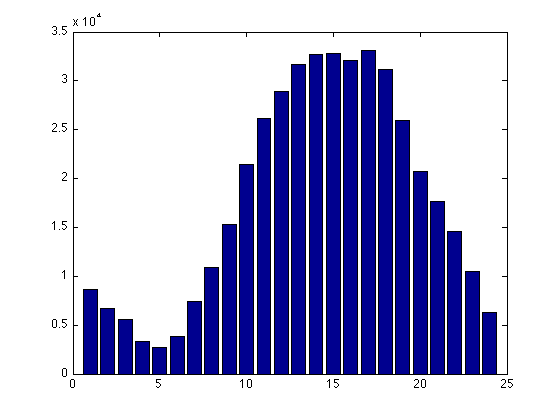
\includegraphics[width=0.45\textwidth]{broncos_off4.png}
			\label{fig:broncos_off}
		}
		\subfigure[] {
			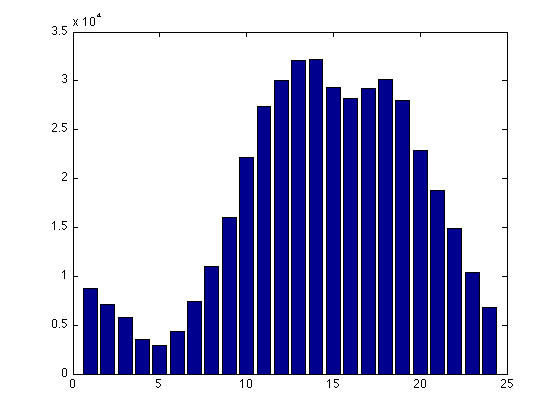
\includegraphics[width=0.45\textwidth]{broncos4.png}
			\label{fig:broncos_on}
		}
	\end{center}
	\caption{Total number of cars passing major highway sensors on Sundays in September and October 2010}
	\label{fig:broncos}
\end{figure}

Such a significant difference in traffic patterns should lead to a change in traffic light control.  We have all encountered the frustrating scenario of attempting to leave one of these sporting events.  Traffic light are often still on predefined timings and the situation arises where a large number of vehicles attempt to get through an traffic light controlled intersection in one direction with almost no vehicles attempting to get through the intersection in the perpendicular direction.  Ideally the light timings should be changed to fix this scenario and increase the green light time in the direction with multiple cars.  Of course, optimally other light timings will also need to be changed to account for the increase volume of traffic along certain paths within the city.

Traditional parametric forecasting models have difficulty accounting for these different traffic patterns and the problem becomes more difficult when when it is considered that the Broncos may play a Sunday night game or a Monday night game.  Thus our another goal of our approach is to handle these significant deviations from normal traffic patterns which are typically the causes of worse case forecasting scenarios.


\subsection{Approach}
To satisfy our first objective of producing an accurate forecast for dataset $x_{t}^(m)$ $\delta$ time steps into the future. We have created an ensemble forecasting model based off of the Bayesian combined forecaster created by Petridis \cite{2001}.  

DISCUSS HOW THIS RELATES TO OBJECTIVE 1
Discuss how we can only show improvements empirically on our work, but that if datasets follow similar structure, we would expect similar results on other data.


THEN disucss we plan to split our approach into two sections, a background model and activity models.  RELATE THIS TO OBJECTIVE 2 here.

We also assume that sufficient deviations from our forecasting function are often not the result of noise, but are due to an activity that does not commonly occur on that day.  Because such activities can overlap or occur at different times with varying amount of background noise present, it is a difficult task for one parametric model to accurately encapsulate all possible combinations of activities.  In an environment with many activities that could occur at multiple different times such combinations may be prevalent.  Past work doesn't address the problem of overlapping activities.  

TODO Create a motivating example off broncos game times residuals with each model
Should tie the introduction together nicely

\begin{figure}{r}{5cm}
	\begin{center}
		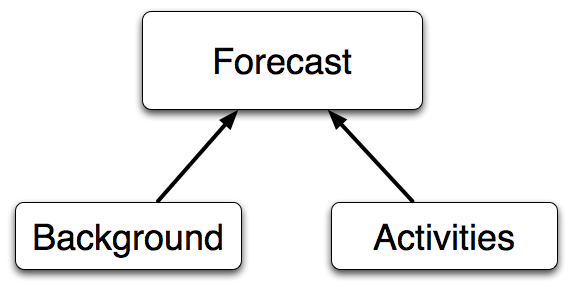
\includegraphics[width=0.30\textwidth]{flow_chart.png}
	\end{center}
	\caption{Forecasting is based on activities and a background model}
	\label{fig:flow_chart}
\end{figure}

Our approach is to split the problem of forecasting into two parts: development of a background model and the development of a set of activity models.  Our background model is represented by a seasonal autoregressive integrated moving average (ARIMA) model.  To model activities, we propose comparing different models from activity recognition literature along with a new model which we propose here.  Forecasting is then performed using an ensemble predictor taking outputs from all trained activity models and the background seasonal ARIMA model. ~\ref{fig:flow_chart}

DISCUSS HOW ALL OF THIS still allows objective 3 to hold.


\subsection{Contributions}  
The contributions to the field of unsupervised traffic forecasting from this work are:
\begin{itemize}
\item{Use of activity models for improved forecasting accuracy of multiple time steps into the future.}
\item{An improvement to a combined Bayesian prediction model to improve forecasting accuracy}
\item{A combined prediction model using an ensemble forecaster and activity models to improve short term forecasts during the presence of anomalous activities}
\end{itemize}

\subsection{Structure of the Proposal}
REDO THE STRUCTURE
The remainder of this proposal is outlined as follows.  Section two reviews current work related to traffic prediction and activity modeling.  Section three gives a summary of each dataset used in this work.  Section four details specific pieces of the overall approach.  All of the approach is not solved and where possible this section details potential ways to proceed with each unsolved part of the approach.  Finally section five is a time line of when the remaining work is expected to be completed.

